% Options for packages loaded elsewhere
\PassOptionsToPackage{unicode}{hyperref}
\PassOptionsToPackage{hyphens}{url}
%
\documentclass[
]{article}
\usepackage{amsmath,amssymb}
\usepackage{iftex}
\ifPDFTeX
  \usepackage[T1]{fontenc}
  \usepackage[utf8]{inputenc}
  \usepackage{textcomp} % provide euro and other symbols
\else % if luatex or xetex
  \usepackage{unicode-math} % this also loads fontspec
  \defaultfontfeatures{Scale=MatchLowercase}
  \defaultfontfeatures[\rmfamily]{Ligatures=TeX,Scale=1}
\fi
\usepackage{lmodern}
\ifPDFTeX\else
  % xetex/luatex font selection
\fi
% Use upquote if available, for straight quotes in verbatim environments
\IfFileExists{upquote.sty}{\usepackage{upquote}}{}
\IfFileExists{microtype.sty}{% use microtype if available
  \usepackage[]{microtype}
  \UseMicrotypeSet[protrusion]{basicmath} % disable protrusion for tt fonts
}{}
\makeatletter
\@ifundefined{KOMAClassName}{% if non-KOMA class
  \IfFileExists{parskip.sty}{%
    \usepackage{parskip}
  }{% else
    \setlength{\parindent}{0pt}
    \setlength{\parskip}{6pt plus 2pt minus 1pt}}
}{% if KOMA class
  \KOMAoptions{parskip=half}}
\makeatother
\usepackage{xcolor}
\usepackage[margin=1in]{geometry}
\usepackage{graphicx}
\makeatletter
\def\maxwidth{\ifdim\Gin@nat@width>\linewidth\linewidth\else\Gin@nat@width\fi}
\def\maxheight{\ifdim\Gin@nat@height>\textheight\textheight\else\Gin@nat@height\fi}
\makeatother
% Scale images if necessary, so that they will not overflow the page
% margins by default, and it is still possible to overwrite the defaults
% using explicit options in \includegraphics[width, height, ...]{}
\setkeys{Gin}{width=\maxwidth,height=\maxheight,keepaspectratio}
% Set default figure placement to htbp
\makeatletter
\def\fps@figure{htbp}
\makeatother
\setlength{\emergencystretch}{3em} % prevent overfull lines
\providecommand{\tightlist}{%
  \setlength{\itemsep}{0pt}\setlength{\parskip}{0pt}}
\setcounter{secnumdepth}{-\maxdimen} % remove section numbering
\ifLuaTeX
  \usepackage{selnolig}  % disable illegal ligatures
\fi
\usepackage{bookmark}
\IfFileExists{xurl.sty}{\usepackage{xurl}}{} % add URL line breaks if available
\urlstyle{same}
\hypersetup{
  pdftitle={Using facet\_ function ( Youtube R101)},
  pdfauthor={Htet Phyo Aung},
  hidelinks,
  pdfcreator={LaTeX via pandoc}}

\title{Using facet\_ function ( Youtube R101)}
\author{Htet Phyo Aung}
\date{2023-07-04}

\begin{document}
\maketitle

\#\#\#Using facets \#\# What are facets

Facets are used to create multiple plots, each showing a subset of your
data. These plots are arranged in a grid, with each plot showing a
different subset of the data, based on the values of one or more
variables. As the saying goes, a picture is worth a thousand words; so
let's look at a a few examples of facets in action.

Let's take a look at the gapminder dataset (that you can access once
you've installed the gapminder package. The variables that are of
interest below are gdpPercap (a crude indicator of a countries wealth)
andlifeExp (which is, as the name suggests, life expectancy).

We're interested in the relationship between these two variables and how
that may vary in different regions of the world. We can see from the
plot below that people living in richer countries do seem to live
longer. It is also clear that that the relationship differs in the
different regions but its difficult to see the details with all of the
plot points overlapping each other.

gapminder \%\textgreater\% filter(gdpPercap \textless{} 40000 \&
continent != ``Oceania'') \%\textgreater\% ggplot(mapping = aes(x =
gdpPercap, y = lifeExp, colour = continent))+ geom\_point(shape =
``square'', alpha = 0.4, size = 2)+ labs(title = ``Life Expectancy as a
function of Wealth'', x = ``GDP per Capita'', y = ``Life Expectancy'',
colour = ``Region'')+ theme\_bw()

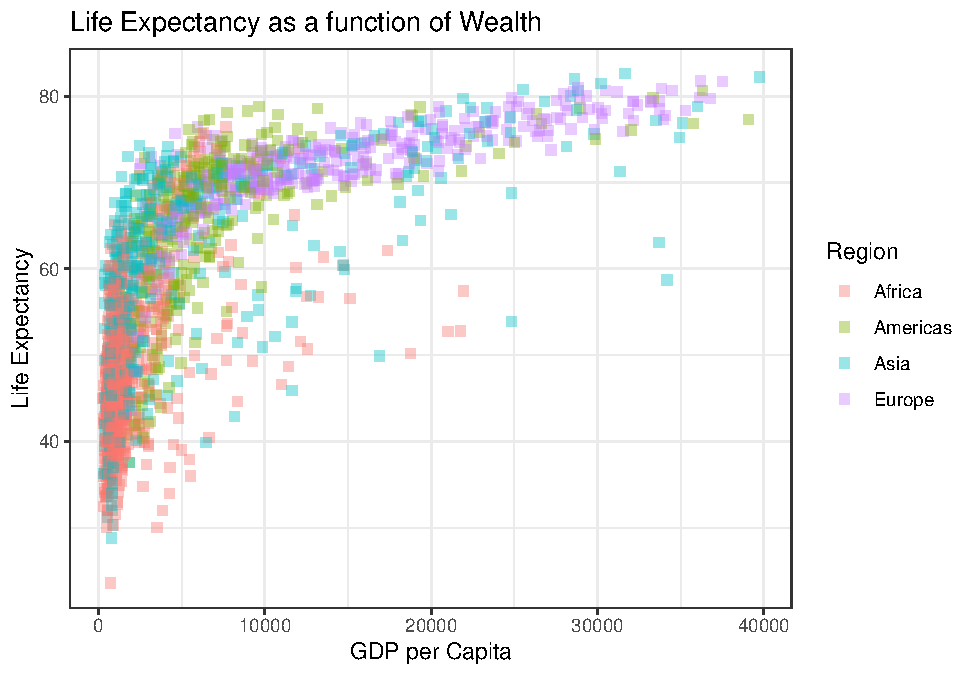
\includegraphics{Using-facet_-function_files/figure-latex/unnamed-chunk-1-1.pdf}

\#\#facet\_wrap

A simple solution is to plot each of the continents of interest on a
separate but adjacent graph so that we can more clearly see the
difference between them. To do this we use the face\_wrap() function and
specify which categorical variable to facet by using the
\textasciitilde{} symbol.

gapminder \%\textgreater\% filter(gdpPercap \textless{} 40000 \&
continent != ``Oceania'') \%\textgreater\% ggplot(mapping = aes(x =
gdpPercap, y = lifeExp, colour = year))+ geom\_jitter(shape =
``square'', alpha = 0.4, size = 2)+ geom\_smooth()+
facet\_wrap(\textasciitilde continent)+ labs(title = ``Life Expectancy
as a function of Wealth'', x = ``GDP per Capita'', y = ``Life
Expectancy'')+ theme\_bw()

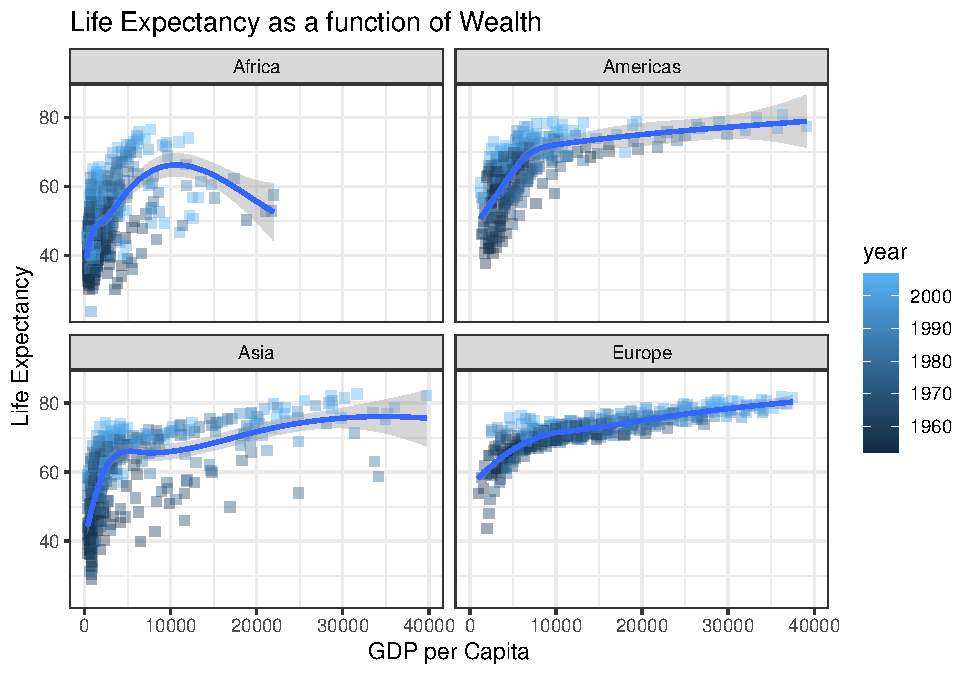
\includegraphics{Using-facet_-function_files/figure-latex/unnamed-chunk-2-1.pdf}

The facet\_wrap function has a number of arguments that can be used to
tweak your plot. Run the command ?facet\_wrap to see a list of all of
the arguments. The more commonly used arguments are nrow and ncol to
specific the number of rows and number of columns respectively. In the
example below, we've used the gss\_cat dataset that comes with the
forcats package to illustrate the use of these arguments. From the
gss\_cat dataset we plot histograms of age, disaggregated by partyid
(political affiliation). To ensure that all of the facets are next to
each other on the same row, we stipulate that nrow = 1. We've also
changed the position of the strip that labels the facet but stipulating
strip.position = ``bottom'':

gss\_cat \%\textgreater\% filter(partyid \%in\% c(``Strong democrat'',
``Strong republican'', ``Independent'')) \%\textgreater\%
ggplot(aes(age))+ geom\_histogram(binwidth = 5, fill = ``steelblue'',
alpha = .8)+ facet\_wrap(\textasciitilde partyid, nrow = 1, ncol = 3,
strip.position = ``bottom'')+ labs(title = ``Age distribution by
political affiliation'', x = ``\,``, y =''\,``)+ theme\_bw()

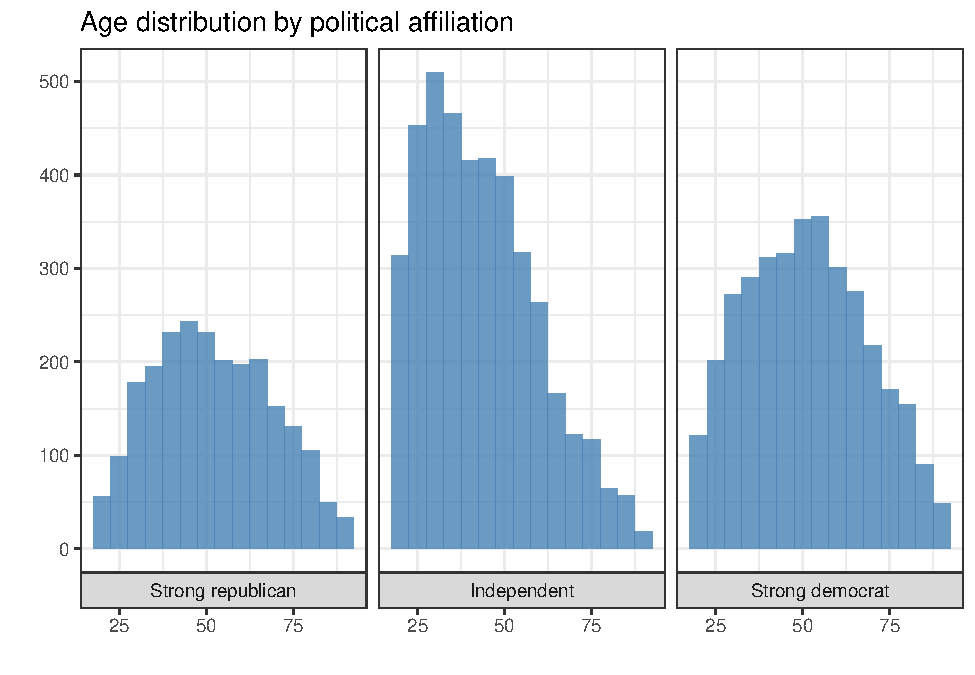
\includegraphics{Using-facet_-function_files/figure-latex/unnamed-chunk-3-1.pdf}

\#\#facet\_grid

Can we facet in two directions? What does that even mean? The easiest
way to describe a facet\_grid is to create one and then take a look at
what it is and how to interpret it. So here we go.

gss\_cat \%\textgreater\% mutate(relig = recode(relig, ``Moslem/islam''
= ``Muslim'')) \%\textgreater\% filter(relig \%in\% c(``Christian'',
``Muslim'') \& partyid \%in\% c(``Strong democrat'',``Strong
republican'', ``Independent'')\& tvhours\textless10) \%\textgreater\%
ggplot(aes(x = tvhours, color = partyid, fill = partyid))+
geom\_density(alpha = 0.3, show.legend = F)+ facet\_grid(relig
\textasciitilde{} partyid)+ labs(title = ``TV watching by political and
religious affiliation'', x = ``Hour spent watching TV'', y = ``\,``)+
theme\_bw()

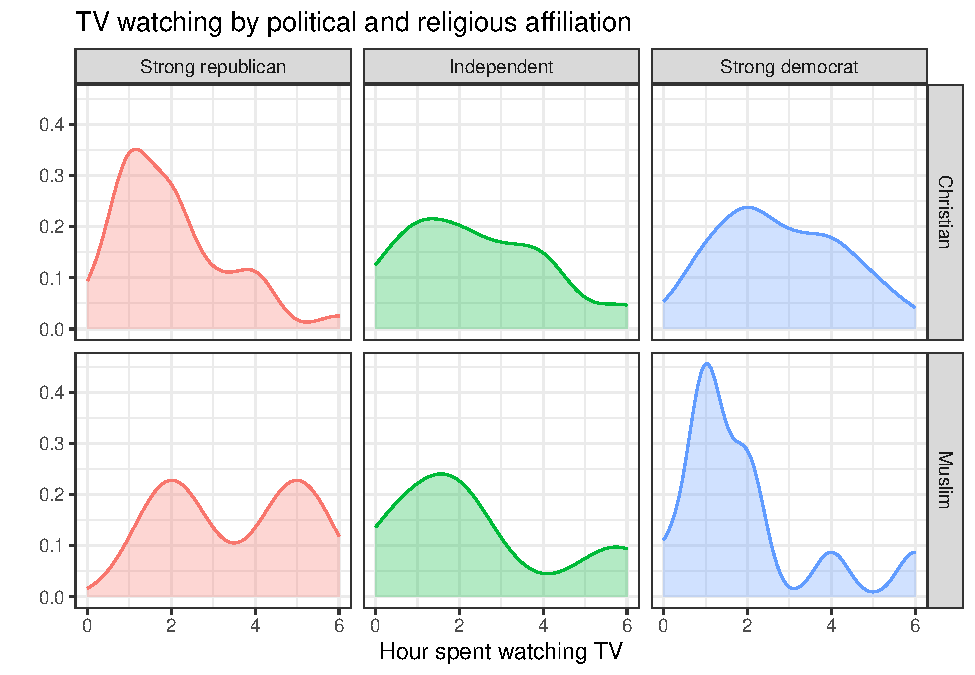
\includegraphics{Using-facet_-function_files/figure-latex/unnamed-chunk-4-1.pdf}

\end{document}
